\subsubsection{Frustration} \label{frust-1}


Die Frustration stellt einen negativen Zustand des Menschen dar, welcher mehrere Indikatoren haben kann. Dieser Zustand kann sowohl eine Gef{\"u}hlslage als auch eine Folge vorhergehender Emotionen sein.
Im Allgemeinen setzt die Frustration ein, wenn Misserfolgserlebnisse sowieVersagungs- und Entt{\"a}uschungserlebnisse vorliegen. 
Ursachen daf{\"u}r k{\"o}nnen in der Person selber und/ oder in Umwelteinfl{\"u}ssen liegen. 
Frustration wird ausgel{\"o}st, wenn die Person eine wirkliche Benachteiligungerleidet oder sie als diese wahrnimmt. 
Eine empfundene Ungerechtigkeit resultierend aus Erwartungen der Umwelt an die Person sowie Erwartungen, die an sich selbst gerichtet sind, k{\"o}nnen den Menschen frustrien. \\

F{\"u}r das Frustrationsexpermiment der Studie soll auf das Ausl{\"o}sen der Misserfolgserlebnisse sowie eine empfundene Ungerechtigkeit zur{\"u}ckgegriffen werden. Der Proband wird aufgefordert das Spiel ``Frustrabit'' zu spielen. 
Ziel des Spiels ist es, den Cursor, mit Hilfe der Computermause, durch das Labyrinth zu navigieren, ohne den Rand bzw die Wand zu ber{\"u}hren. 
Hinzu kommt die Aufgabenstellung, acht Level  innerhalb von f{\"u}nf Minuten zu l{\"o}sen, um eine Pr{\"a}mie von 10 EUR zu gewinnen.
Zur Manipulation hat der Versuchsleiter eine kabellose Maus, von der der Proband nichts wei{\ss}. 
Mit Hilfe dieser Maus verhindert der Versuchsleiter, dass der Proband die Aufgabenstellung erf{\"u}llen und die Pr{\"a}mie gewinnen kann, indem der Versuchsleiter den Cursor nach belieben an die Wand des Labyrinths steuert. 


\begin{figure}[H] \centering
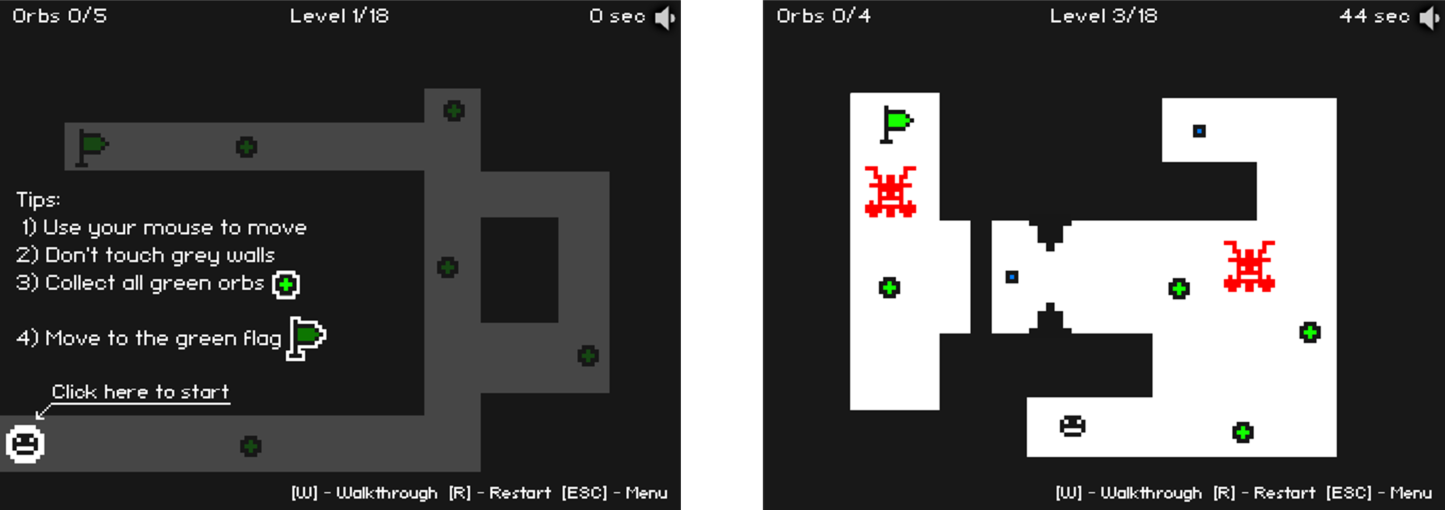
\includegraphics[width=\textwidth]{Images/frustabit.png} 
\vspace{-0.3cm} 
\caption{Bild des Frustabit Spieles für das Frustration-Szenario.}
\label{fig-frust} 
\end{figure}